% Options for packages loaded elsewhere
\PassOptionsToPackage{unicode}{hyperref}
\PassOptionsToPackage{hyphens}{url}
%
\documentclass[
]{book}
\usepackage{amsmath,amssymb}
\usepackage{lmodern}
\usepackage{ifxetex,ifluatex}
\ifnum 0\ifxetex 1\fi\ifluatex 1\fi=0 % if pdftex
  \usepackage[T1]{fontenc}
  \usepackage[utf8]{inputenc}
  \usepackage{textcomp} % provide euro and other symbols
\else % if luatex or xetex
  \usepackage{unicode-math}
  \defaultfontfeatures{Scale=MatchLowercase}
  \defaultfontfeatures[\rmfamily]{Ligatures=TeX,Scale=1}
\fi
% Use upquote if available, for straight quotes in verbatim environments
\IfFileExists{upquote.sty}{\usepackage{upquote}}{}
\IfFileExists{microtype.sty}{% use microtype if available
  \usepackage[]{microtype}
  \UseMicrotypeSet[protrusion]{basicmath} % disable protrusion for tt fonts
}{}
\makeatletter
\@ifundefined{KOMAClassName}{% if non-KOMA class
  \IfFileExists{parskip.sty}{%
    \usepackage{parskip}
  }{% else
    \setlength{\parindent}{0pt}
    \setlength{\parskip}{6pt plus 2pt minus 1pt}}
}{% if KOMA class
  \KOMAoptions{parskip=half}}
\makeatother
\usepackage{xcolor}
\IfFileExists{xurl.sty}{\usepackage{xurl}}{} % add URL line breaks if available
\IfFileExists{bookmark.sty}{\usepackage{bookmark}}{\usepackage{hyperref}}
\hypersetup{
  pdftitle={ENG 792 - Análise e visualização de dados com R (RStudio)},
  pdfauthor={Jackson Rodrigues},
  hidelinks,
  pdfcreator={LaTeX via pandoc}}
\urlstyle{same} % disable monospaced font for URLs
\usepackage{color}
\usepackage{fancyvrb}
\newcommand{\VerbBar}{|}
\newcommand{\VERB}{\Verb[commandchars=\\\{\}]}
\DefineVerbatimEnvironment{Highlighting}{Verbatim}{commandchars=\\\{\}}
% Add ',fontsize=\small' for more characters per line
\usepackage{framed}
\definecolor{shadecolor}{RGB}{248,248,248}
\newenvironment{Shaded}{\begin{snugshade}}{\end{snugshade}}
\newcommand{\AlertTok}[1]{\textcolor[rgb]{0.94,0.16,0.16}{#1}}
\newcommand{\AnnotationTok}[1]{\textcolor[rgb]{0.56,0.35,0.01}{\textbf{\textit{#1}}}}
\newcommand{\AttributeTok}[1]{\textcolor[rgb]{0.77,0.63,0.00}{#1}}
\newcommand{\BaseNTok}[1]{\textcolor[rgb]{0.00,0.00,0.81}{#1}}
\newcommand{\BuiltInTok}[1]{#1}
\newcommand{\CharTok}[1]{\textcolor[rgb]{0.31,0.60,0.02}{#1}}
\newcommand{\CommentTok}[1]{\textcolor[rgb]{0.56,0.35,0.01}{\textit{#1}}}
\newcommand{\CommentVarTok}[1]{\textcolor[rgb]{0.56,0.35,0.01}{\textbf{\textit{#1}}}}
\newcommand{\ConstantTok}[1]{\textcolor[rgb]{0.00,0.00,0.00}{#1}}
\newcommand{\ControlFlowTok}[1]{\textcolor[rgb]{0.13,0.29,0.53}{\textbf{#1}}}
\newcommand{\DataTypeTok}[1]{\textcolor[rgb]{0.13,0.29,0.53}{#1}}
\newcommand{\DecValTok}[1]{\textcolor[rgb]{0.00,0.00,0.81}{#1}}
\newcommand{\DocumentationTok}[1]{\textcolor[rgb]{0.56,0.35,0.01}{\textbf{\textit{#1}}}}
\newcommand{\ErrorTok}[1]{\textcolor[rgb]{0.64,0.00,0.00}{\textbf{#1}}}
\newcommand{\ExtensionTok}[1]{#1}
\newcommand{\FloatTok}[1]{\textcolor[rgb]{0.00,0.00,0.81}{#1}}
\newcommand{\FunctionTok}[1]{\textcolor[rgb]{0.00,0.00,0.00}{#1}}
\newcommand{\ImportTok}[1]{#1}
\newcommand{\InformationTok}[1]{\textcolor[rgb]{0.56,0.35,0.01}{\textbf{\textit{#1}}}}
\newcommand{\KeywordTok}[1]{\textcolor[rgb]{0.13,0.29,0.53}{\textbf{#1}}}
\newcommand{\NormalTok}[1]{#1}
\newcommand{\OperatorTok}[1]{\textcolor[rgb]{0.81,0.36,0.00}{\textbf{#1}}}
\newcommand{\OtherTok}[1]{\textcolor[rgb]{0.56,0.35,0.01}{#1}}
\newcommand{\PreprocessorTok}[1]{\textcolor[rgb]{0.56,0.35,0.01}{\textit{#1}}}
\newcommand{\RegionMarkerTok}[1]{#1}
\newcommand{\SpecialCharTok}[1]{\textcolor[rgb]{0.00,0.00,0.00}{#1}}
\newcommand{\SpecialStringTok}[1]{\textcolor[rgb]{0.31,0.60,0.02}{#1}}
\newcommand{\StringTok}[1]{\textcolor[rgb]{0.31,0.60,0.02}{#1}}
\newcommand{\VariableTok}[1]{\textcolor[rgb]{0.00,0.00,0.00}{#1}}
\newcommand{\VerbatimStringTok}[1]{\textcolor[rgb]{0.31,0.60,0.02}{#1}}
\newcommand{\WarningTok}[1]{\textcolor[rgb]{0.56,0.35,0.01}{\textbf{\textit{#1}}}}
\usepackage{longtable,booktabs,array}
\usepackage{calc} % for calculating minipage widths
% Correct order of tables after \paragraph or \subparagraph
\usepackage{etoolbox}
\makeatletter
\patchcmd\longtable{\par}{\if@noskipsec\mbox{}\fi\par}{}{}
\makeatother
% Allow footnotes in longtable head/foot
\IfFileExists{footnotehyper.sty}{\usepackage{footnotehyper}}{\usepackage{footnote}}
\makesavenoteenv{longtable}
\usepackage{graphicx}
\makeatletter
\def\maxwidth{\ifdim\Gin@nat@width>\linewidth\linewidth\else\Gin@nat@width\fi}
\def\maxheight{\ifdim\Gin@nat@height>\textheight\textheight\else\Gin@nat@height\fi}
\makeatother
% Scale images if necessary, so that they will not overflow the page
% margins by default, and it is still possible to overwrite the defaults
% using explicit options in \includegraphics[width, height, ...]{}
\setkeys{Gin}{width=\maxwidth,height=\maxheight,keepaspectratio}
% Set default figure placement to htbp
\makeatletter
\def\fps@figure{htbp}
\makeatother
\setlength{\emergencystretch}{3em} % prevent overfull lines
\providecommand{\tightlist}{%
  \setlength{\itemsep}{0pt}\setlength{\parskip}{0pt}}
\setcounter{secnumdepth}{5}
\usepackage{booktabs}
\ifluatex
  \usepackage{selnolig}  % disable illegal ligatures
\fi
\usepackage[]{natbib}
\bibliographystyle{plainnat}

\title{ENG 792 - Análise e visualização de dados com R (RStudio)}
\author{Jackson Rodrigues}
\date{2021-08-10}

\begin{document}
\maketitle

{
\setcounter{tocdepth}{1}
\tableofcontents
}
\hypertarget{apresentauxe7uxe3o}{%
\chapter{Apresentação}\label{apresentauxe7uxe3o}}

\hypertarget{hello-world---sejam-bem-vindos}{%
\section{Hello World! - Sejam Bem Vindos!}\label{hello-world---sejam-bem-vindos}}


\includegraphics[width=0.5\textwidth,height=0.5\textheight]{J:/ENG 792/ENG_792-AVDR/ENG.792-AVDR/Cap_1_ET.jpg}

Este é o material para os alunos matriculados na disciplina \textbf{ENG 792 - Análise e Visualização de dados com R (RStudio)} ofertada pelo programa de pós-graduação em Meteorologia Aplicada da Universidade Federal de Viçosa (UFV).

Este curso foi criado e é ministrado por Jackson Rodrigues, professor da Universidade Federal Fluminense (UFF), mas também professor no programa de pós-graduação em Meteorologia Aplicada do Departamento de Engenharia Agrícola (DEA) da Universidade Federal de Viçosa (UFV).

Este curso foi construído pensando em minha saga para aprender algo utilizando o R em meu doutorado. Foi bastante dolorido, principalmente no começo quando eu nunca havia tido contato com a liguagem, na verdade, sabia quase nada em programação.

Desta forma, o público alvo é aquele que tem conhecimento

zero

sobre o assunto. Mas se você já sabe algo em qualquer nível, seja bem vindo também e podemos aprender juntos, você ensina o que você sabe e eu ensino o que eu sei.

A ideia principal deste curso é que o(a) aluno(a) que nada sabe de \textbf{R} seja exposto(a) a grande quantidade de conceitos e métodos para que o ``gelo'' seja quebrado e possa se virar sozinho ao término do curso. Desta forma, não é um curso de estatística, não é um curso de produção gráfica nem um curso produção de conteúdo (eg. modelagem), mas um curso de exposição, quase um ``\emph{how to}''. Vamos levantar demandas do dia a dia e tentar resolver os problemas comuns enfrentados pelo estudante na condução de suas análises.

Eventualmente algum especialista será convidado para dar uma aula, bater um papo, fazer uma apresentação e etc sobre um assunto específico.

O R é uma ferramenta espetacular para análise e produção de dados, bem como produção gráfica! Vamos começar devagar e ao poucos vocês vão se tornando autossuficientes.
Muitas dúvidas surgem em fóruns, grupos e tanto outros canais de comunicação da comunidade de usuários de R.

Muitas vezes surgem perguntas como:

``Tem como fazer isso no R?''

A resposta imediada, devido à sua versatilidade, é:

``A pergunta não é''se tem jeito``, mas''como fazer".

Vamos dar uma passeio por muitas coisas legais que o \textbf{R} pode fazer e que vão ajudar a tornar sua vida bem melhor. Com tempo ganho na otimização das suas tarefas por utilização do \textbf{R} sobrará tempo para você escrever um paper a mais na pós-graduação, dormir no final de semana sem culpa, tomar uma cerveja na sexta com a turma e ir ao culto domingo sem pedidos.

Vamos fazer tudo isso nos divertindo. É legal! Vocês verão. Por isso não se procupem comigo (professor), será muito pior para mim por ter que corrigir trabalhos enquanto vocês produzem mais um paper, dormem, tomam um cerveja com a turma e/ou rezam como foi na véspera de natal de 2020 quando estava corrigindo trabalhos.

\begin{figure}
\hypertarget{id}{%
\centering
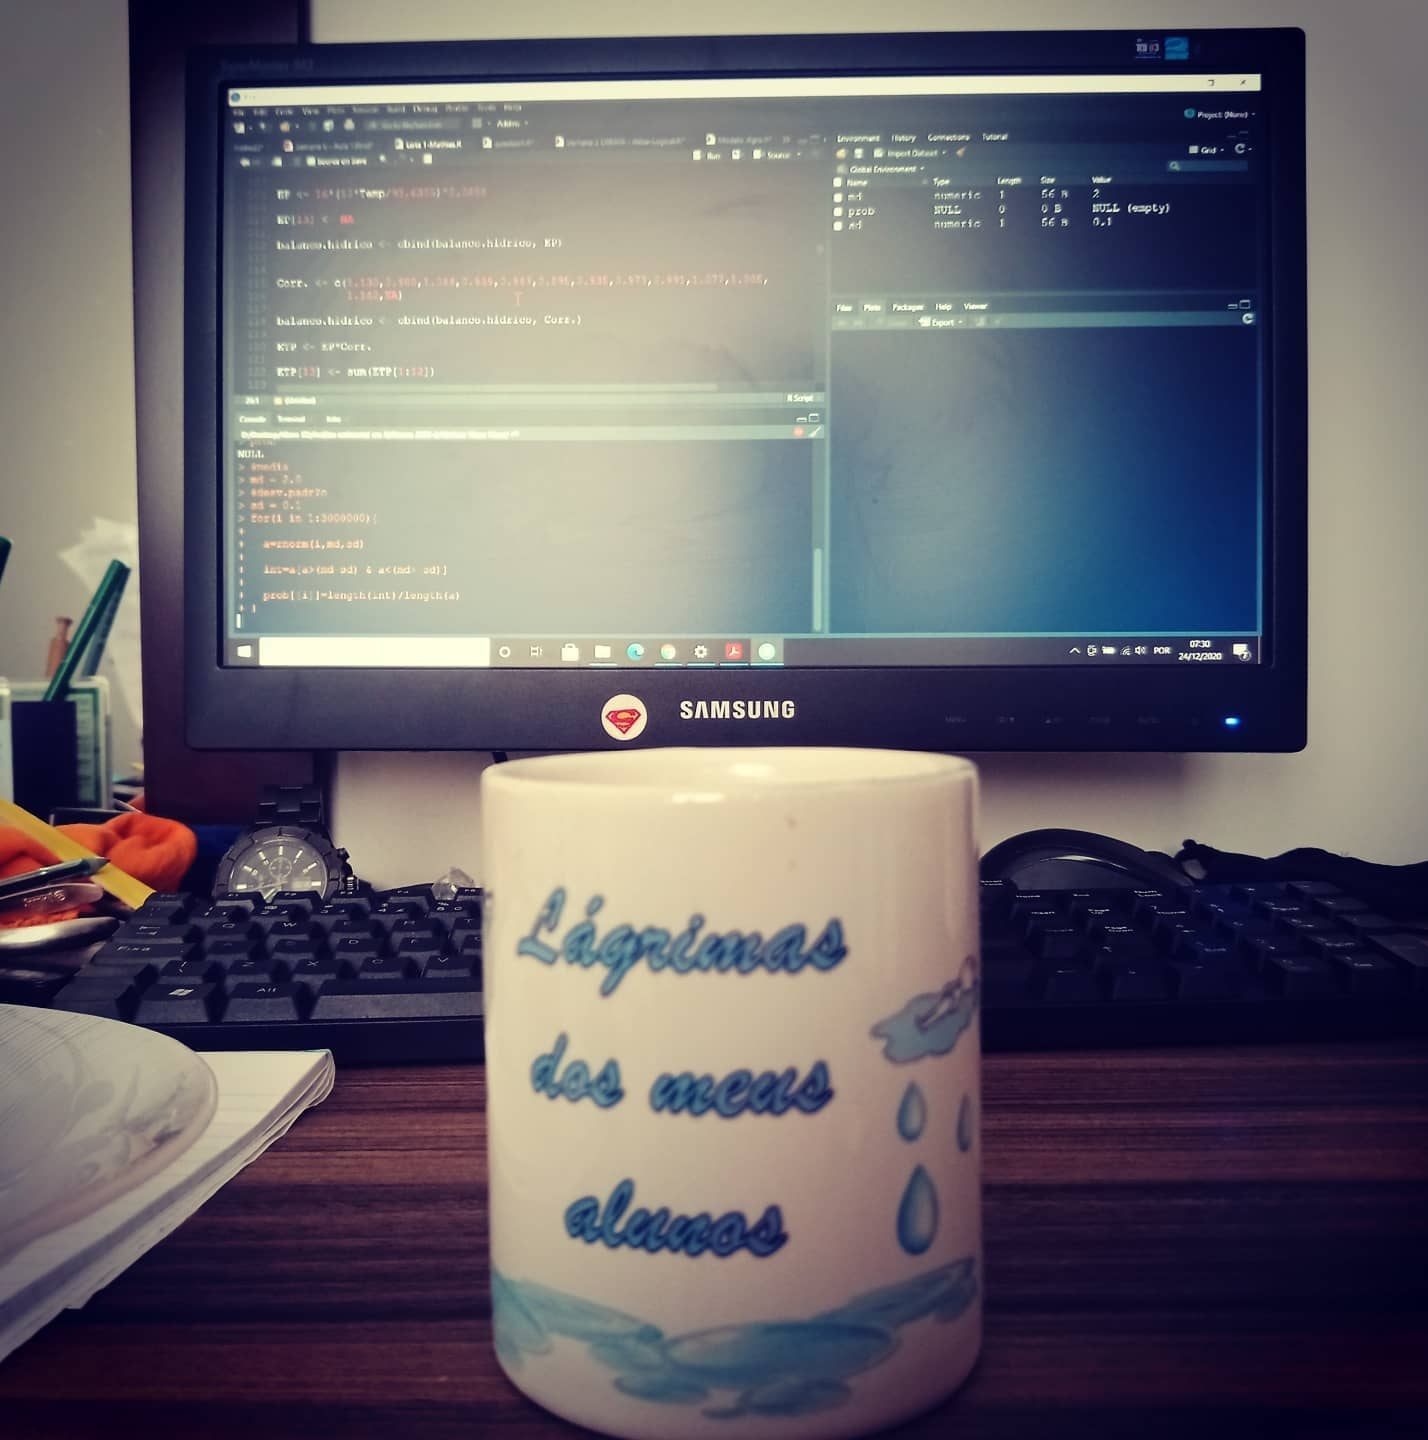
\includegraphics[width=0.7\textwidth,height=0.7\textheight]{J:/ENG 792/ENG_792-AVDR/ENG.792-AVDR/Cap_1_Vespera_de_Natal.jpg}
\caption{Véspera de Natal 2020}\label{id}
}
\end{figure}

\href{https://www.youtube.com/watch?v=N8E4s8yAoX4\&ab_channel=MassacrationOficial}{Let's ride to Metal Land!}

Nâo se sintam pressionados ou intimidados, façam as perguntas que quiserem. Eu também não sei tudo, o R é uma ferramenta que está em constante desenvolvimento tornando impossível acompanhar cada novidade. Caso eu não saiba uma resposta não tenho problemas em dizer que não sei, mas vou me esforçar para buscar a resposta.

Por isso:

\begin{itemize}
\item
  Vamos aprender e tentar nos divertir;
\item
  Pensei nesse curso como uma forma de lutar contra a ``dor'' que senti quando comecei a trabalhar no R sozinho;
\item
  Então sou um usuário e não um programador;
\item
  A verdade é que o R tem uma curva de aprendizado muito íngreme que uma vez vencido o primeiro obstáculo as coisas deslancham;
\item
  Vamos trabalhar de maneira que esse curso atenda superficialmente suas demandas e que te habilitem a se virarem sozinhos;
\item
  Então vamos seguir passo-a-passo para um aprendizado gradual com vários exemplos;
\item
  Tudo que você aprender em determinando momento não será descartado, você deverá guardar aquele conhecimento para utilização em próximo trabalho ou tarefa;
\item
  Ou ainda, este conhecimento inicial será utilizado para sedimentar o caminho para um próximo passo;
\item
  Aplicar o máximo possível nosso conhecimento a problemas reais, do mundo real.
\end{itemize}

Para finalizar gostaria de deixar algumas coisas claras.

\begin{itemize}
\item
  Este curso conta com vasto material encontrado em artigos, livros, blogs especializados, grupos de discussões e etc. Desta forma, caso encontre por aí algo que ofertei em aula não precisa me chamar de picareta. Provavelmente foi tirado de lá mesmo.
\item
  O curso funciona como um \textbf{\emph{How to}}. Não teremos tempo de nos aprofundar nas teorias dos assuntos aqui apresentados (nem é a intenção), por isso, vou mostrar o \textbf{``que é''}, \textbf{``como usar''} e \textbf{``como fazer''}.
\item
  Ao término de cada aula será mostrada uma bibliografia básica sobre o conteúdo. Como são conteúdos diversificados, acho melhor separar as bibliografias por aula.
\end{itemize}

\hypertarget{sobre}{%
\subsection{Sobre}\label{sobre}}

Este é um material de apoio compilado e criado para os alunos da disciplina \textbf{ENG 792 - Análise e visualização de dados com R (RStudio)}.

Importante mencionar que o conteúdo aqui apresentado é um compilado de vários anos de materiais estudados disponíveis \emph{online} ou em livros e artigos especialzados. Desta forma, caso identifique algum conteúdo apresentado aqui que não esteja devidamente referenciado fique à vontade para solicitar os devidos créditos aos autores originais. Não tenho a intenção de ter crédito que não é meu.

\hypertarget{utilizauxe7uxe3o}{%
\subsection{Utilização}\label{utilizauxe7uxe3o}}

Cada capítulo é referente ao conteúdo de mais ou menos uma semana de curso. Cada semama trata de um assunto diferente e complementar ao conteúdo da semana anterior.
Desta forma, fique livre para ir e vir no conteúdo caso algo não esteja claro o suficiente.

\begin{itemize}
\tightlist
\item
  Teremos aulas gravadas e aulas síncronas através de alguma plataforma.\\
\item
  Apenas os alunos matriculados na disciplina terão acesso ao conteúdo gravado.\\
\item
  A distribuição e/ou compartilhamento do conteúdo gravado por qualquer meio é proibido.
\end{itemize}

\hypertarget{cuxf3digos-e-dados}{%
\subsection{Códigos e Dados}\label{cuxf3digos-e-dados}}

Todo o material necessário para acompanhar a disciplina será oferecido via \href{https://github.com/Jacksonmrod/ENG-792}{github}. Os códigos com alguma explicação neste material online (explicação completa nas aulas) e os dados onde forem possíveis de serem armazenados.

\hypertarget{cronograma-de-aulas}{%
\subsection{Cronograma de aulas}\label{cronograma-de-aulas}}

As aulas serão ofertadas por material gravado e presencial às quintas e sextas entre 14:00 e 15:30.

\begin{longtable}[]{@{}
  >{\centering\arraybackslash}p{(\columnwidth - 2\tabcolsep) * \real{0.12}}
  >{\centering\arraybackslash}p{(\columnwidth - 2\tabcolsep) * \real{0.88}}@{}}
\toprule
Semana & Conteúdo \\
\midrule
\endhead
1.1 & Apresentação do Conteúdo e Instalação do R \\
1.2 & Funcionamento do R, tipo e estrutura dos objetos \\
2.1 & Manipulação de dados 1 \\
2.2 & Manipulação de dados 2, testes lógicos e simbolos, condicionais e interações \\
3.1 & Pacotes e Funções \\
3.2 & Entrando/Importando dados. definição de diretórios \\
4.1 & Produção gráfica com Rbase \\
4.2 & Produção gráfica com ggplot 2 \\
5.1 & Elementos de estatística básica 1 (Est. Descritiva, Med. Tend. Central, Medi. de variabilidade) \\
5.2 & Elementos de estatítica básica 2 (Dife. Entre médias, T-Student, Teste F, Testes de normalidade) \\
6.1 & Elementos de estatítica básica 3 (ANOVA, delineamento, comparaçõe múltiplas, Regressão, Resíduos, Homocedasticidade, Normalidade dos resíduos, regressão múltipla, superfície de resposta) \\
7.1 & Análise Multivariada (Análise de agrupamento, medidas de (dis)similaridade, métodos de conexão, número de clusters, produção de dendogramas, árvores de decisão) \\
7.2 & Métodos de Ordenação (Ana. Componentes Principais, Análise Canônica, Análise de fatores, Análise de Mahalanobis) \\
8 - 15 & Será preenchido em breve \\
\bottomrule
\end{longtable}

\hypertarget{muxe9todos-de-avaliauxe7uxe3o}{%
\subsection{Métodos de avaliação}\label{muxe9todos-de-avaliauxe7uxe3o}}

\begin{itemize}
\tightlist
\item
  Faremos pelo menos 3 listas de exercícios distribuídas pelo semestre.\\
\item
  O trabalho final será a confecção de um atrabalho autoral com o conteúdo do curso que poderá ser feito em grupo (isso será definido ainda em conversa com vocês). Este trabalho será apresentado na forma de seminário ao término do curso.
\end{itemize}

\hypertarget{vamos-ao-que-interesa}{%
\chapter{Vamos ao que interesa}\label{vamos-ao-que-interesa}}

\hypertarget{conhecendo-o-r}{%
\section{Conhecendo o R}\label{conhecendo-o-r}}

\hypertarget{o-que-uxe9-o-r}{%
\subsection{O que é o R?}\label{o-que-uxe9-o-r}}

É uma linguagem de programação voltada para resolução de problemas estatísticos, tratamento e visualização de dados.

Para \citet{RogerPeng2020RPro} essa resposta é simples, ``\emph{R é um dialeto do S}''.

De acordo com \citet{perlin2018processamento} \emph{O código base do R foi inicialmente criado no laboratório da Bell/ AT\& T por John Chambers e seus colegas, com base na linguagem S. Esse código foi reaproveitado por dois acadêmicos, Ross Ihaka e Robert Gentleman, resultando na plataforma de programação que temos hoje. Para os curiosos, o nome R foi escolhido devido ao compartilhamento da primeira letra do nome de seus criadores.}

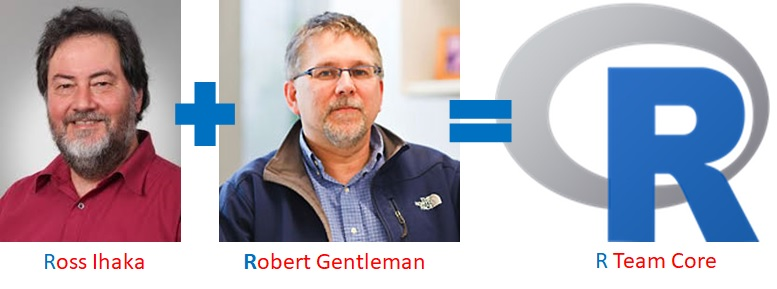
\includegraphics[width=0.7\textwidth,height=0.7\textheight]{J:/ENG 792/ENG_792-AVDR/ENG.792-AVDR/Cap_1_Ross_Robert R.jpg}

O R está em constante desenvolvimento por um grupo chamado \href{https://www.r-project.org/}{R Team Core} e conta com colaboração gratuita de centenas de milhares de usuários e desenvolvedores ao redor do mundo.
Por isso, atualmente o R é utilizado por diversas áreas do conhecimento variando das ciências humanas até exatas, naquelas ciências que poderíamos imaginar pouco ou nada relacionadas. Por isso não se limite a procurar informações apenas no sei nicho, abra sua mente e busque aprender de outras ciências também. Eu, particularmente, busco muita coisa na econometria. embora presente em todo tipo de livro sobre R, asta citação acima (\citet{perlin2018processamento}) é de um livro de econometria. Veremos mais conteúdos desse material em breve.

R é um software livre de análise de dados (não só estatística) que funciona em diversos sistemas operacionais: GNU Linux, MicrosoftWindows, Mac OS X e outros.

O aprendizado do R é difícil no início devido à necessidade de se adaptar à sua lógica de funcionamento, se acostumar com a estrutura dos seus documentos de ajuda e memorizar alguns comandos básicos.

\begin{Shaded}
\begin{Highlighting}[]
\NormalTok{eq }\OtherTok{=} \ControlFlowTok{function}\NormalTok{(x)\{x}\SpecialCharTok{*}\NormalTok{x\}}
\FunctionTok{plot}\NormalTok{(}\FunctionTok{eq}\NormalTok{(}\DecValTok{1}\SpecialCharTok{:}\DecValTok{1000}\NormalTok{), }\AttributeTok{type=}\StringTok{"l"}\NormalTok{,}\AttributeTok{lwd=}\DecValTok{3}\NormalTok{,}\AttributeTok{col=}\StringTok{"red"}\NormalTok{, }\AttributeTok{xaxt=}\StringTok{"n"}\NormalTok{, }\AttributeTok{yaxt=}\StringTok{"n"}\NormalTok{, }\AttributeTok{xlab=}\StringTok{"Tempo"}\NormalTok{, }\AttributeTok{ylab=}\StringTok{"Aprendizado"}\NormalTok{, }\AttributeTok{main=}\StringTok{"Curva de Aprendizado"}\NormalTok{)}
\end{Highlighting}
\end{Shaded}

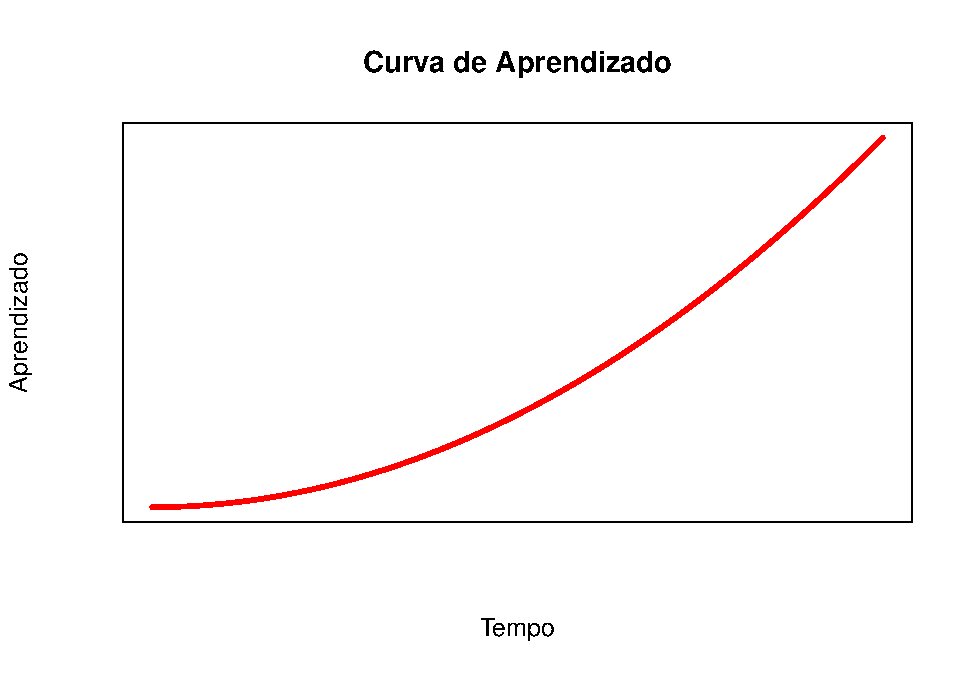
\includegraphics{ENG_792-AVDR_files/figure-latex/CurvaR-1.pdf}

É preciso bastante perseverança e motivação para aprender os comandos básicos, e disposição para ler as páginas de ajuda e os manuais.
Entretanto, depois de um certo tempo, ele possibilita que se trabalhe com grande produtividade e, o que é mais importante, eficácia e independência.

Leia também sobre o \href{https://www.r-bloggers.com/2021/07/the-myth-of-the-r-learning-curve/}{mito da curva de aprendizado do R}.

\hypertarget{instalauxe7uxe3o-do-r}{%
\subsection{Instalação do R}\label{instalauxe7uxe3o-do-r}}

O \textbf{R} é um software gratuito para análises estatísticas e além. Pode ser baixado de \href{https://www.r-project.org/}{The R Project for Statistical Computing}.

Clique em \textbf{download R}.\\
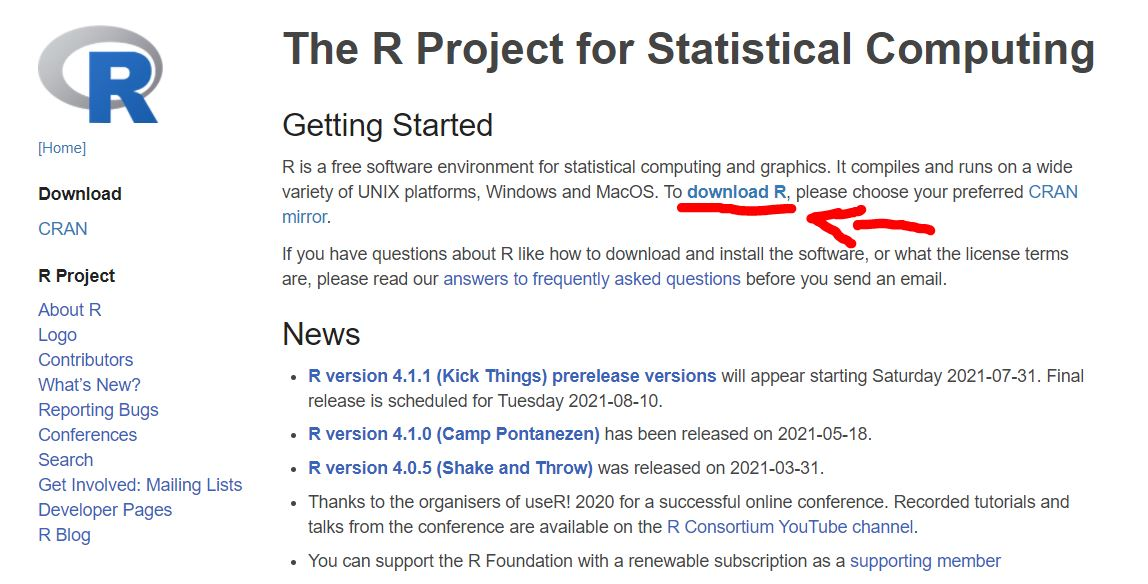
\includegraphics[width=0.9\textwidth,height=0.9\textheight]{J:/ENG 792/ENG_792-AVDR/ENG.792-AVDR/Cap_1_Pagina_R.jpg}

Escolha o \emph{``espelho''}.Escolha o mais próximo de você.\\

\includegraphics[width=0.9\textwidth,height=0.9\textheight]{J:/ENG 792/ENG_792-AVDR/ENG.792-AVDR/Cap_1_Pagina_R_MIrror.jpg}

Escolha o seu sistema operacional. Caso você seja usuário de windows clique em \textbf{Download R for Windows} em seguinda em \textbf{install R for the first time} e finalmente em \textbf{Download R 4.1.0 for Windows}. Veja que no momento que este tutorial foi feito a versdão mais recente é a 4.1.0. No vídeo abaixo a versão é uma anterior, mas a lógica é a mesma.\\
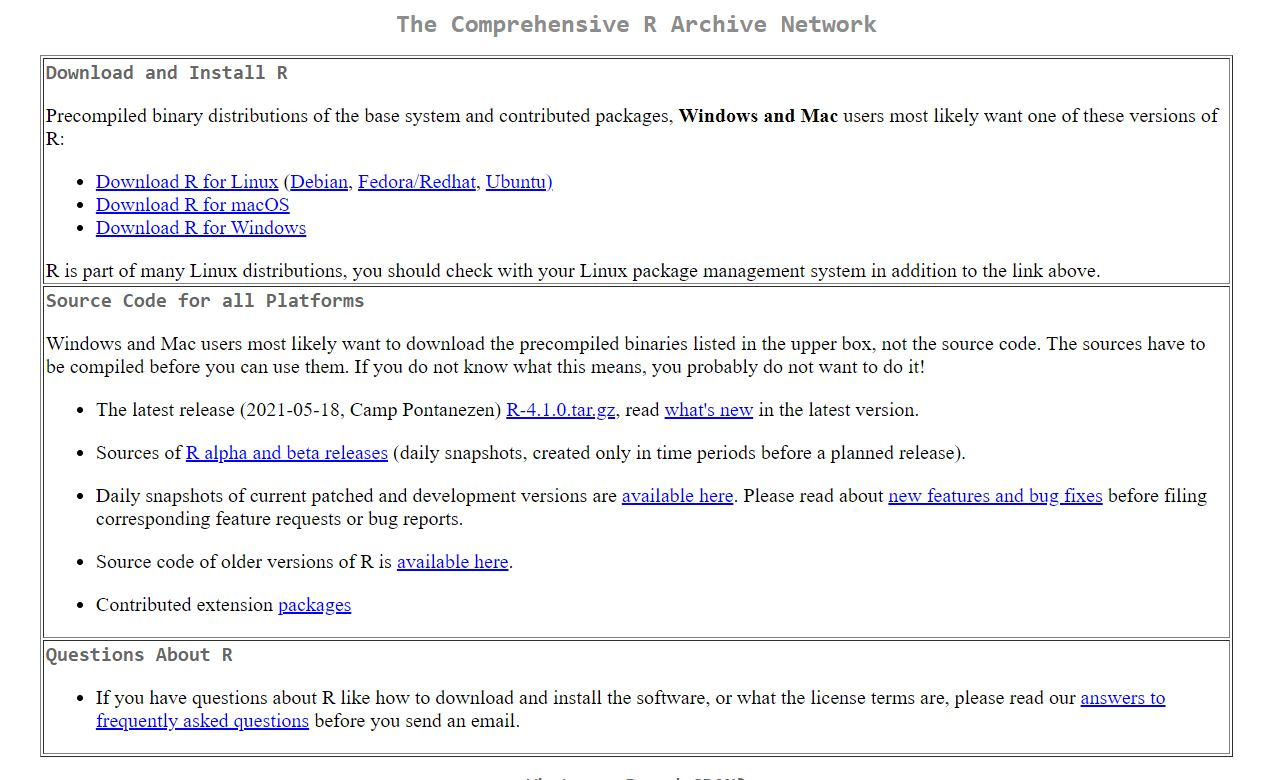
\includegraphics[width=0.9\textwidth,height=0.9\textheight]{J:/ENG 792/ENG_792-AVDR/ENG.792-AVDR/Cap_1_Pagina_R_sistema_operacional.jpg}

\href{https://sites.google.com/d/1eCt5C338czwUdwb5R-3k98vHFdf5LFC7/p/1l-WXVHDr8j6cYk-iTSYBaFN7mTesOmQl/edit}{clique aqui} para assistir ao vídeo de instalação do R e RStudio no windows

Eu não tenho um sistema operacional de cada para mostrar a instalação, por isso deixo este vídeo para \href{https://www.youtube.com/watch?v=np2-FIgzpTg\&ab_channel=AutoDeeDucks}{instalação no linux} e este para \href{https://www.youtube.com/watch?v=LanBozXJjOk\&ab_channel=DataSciencewithTom}{instalação no mac}. Caso você não consiga instalar me procure.

\hypertarget{primeiro-contato}{%
\subsection{Primeiro contato}\label{primeiro-contato}}

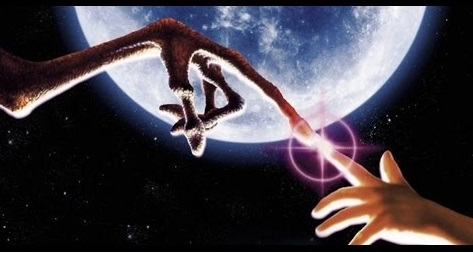
\includegraphics[width=0.5\textwidth,height=0.5\textheight]{J:/ENG 792/ENG_792-AVDR/ENG.792-AVDR/Cap_1_ET-dedo.jpg}

Temos 1 arquivo .csv com mais de 50.000 linhas referentes a transações de venda de diamantes dividida em 3 colunas \emph{clarity}, \emph{carat} e \emph{price}. Quanto mais claro mais caro, certo? Ou há sub ou super valorização? Vamos investigar se essa relação é verdadeira.

\begin{Shaded}
\begin{Highlighting}[]
\NormalTok{mydata}\OtherTok{\textless{}{-}}\FunctionTok{read.csv}\NormalTok{(}\StringTok{"J:/ENG 792/ENG\_792{-}AVDR/ENG.792{-}AVDR/Cap\_1\_P2{-}Mispriced{-}Diamonds.csv"}\NormalTok{)}

\FunctionTok{library}\NormalTok{(}\StringTok{"ggplot2"}\NormalTok{)}
\FunctionTok{ggplot}\NormalTok{(}\AttributeTok{data=}\NormalTok{mydata, }\FunctionTok{aes}\NormalTok{(}\AttributeTok{x=}\NormalTok{carat, }\AttributeTok{y=}\NormalTok{price))}\SpecialCharTok{+} 
  \FunctionTok{geom\_point}\NormalTok{()}
\end{Highlighting}
\end{Shaded}

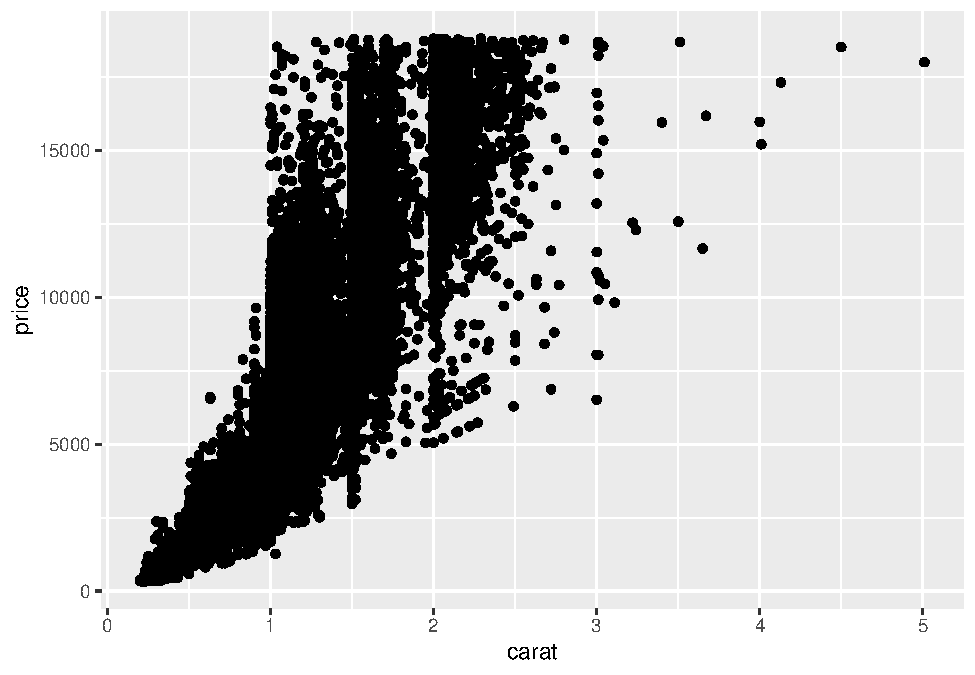
\includegraphics{ENG_792-AVDR_files/figure-latex/Exemplo_1-1.pdf}
Faz algum sentido. Mas temos pontos que não são estatisticamente significantes à direita, então vamos fazer uma limpeza, vamos mexer na transparência.

\begin{Shaded}
\begin{Highlighting}[]
\FunctionTok{ggplot}\NormalTok{(}\AttributeTok{data=}\NormalTok{mydata, }\FunctionTok{aes}\NormalTok{(}\AttributeTok{x=}\NormalTok{carat, }\AttributeTok{y=}\NormalTok{price, }\AttributeTok{colour=}\NormalTok{clarity))}\SpecialCharTok{+} 
  \FunctionTok{geom\_point}\NormalTok{()}
\end{Highlighting}
\end{Shaded}

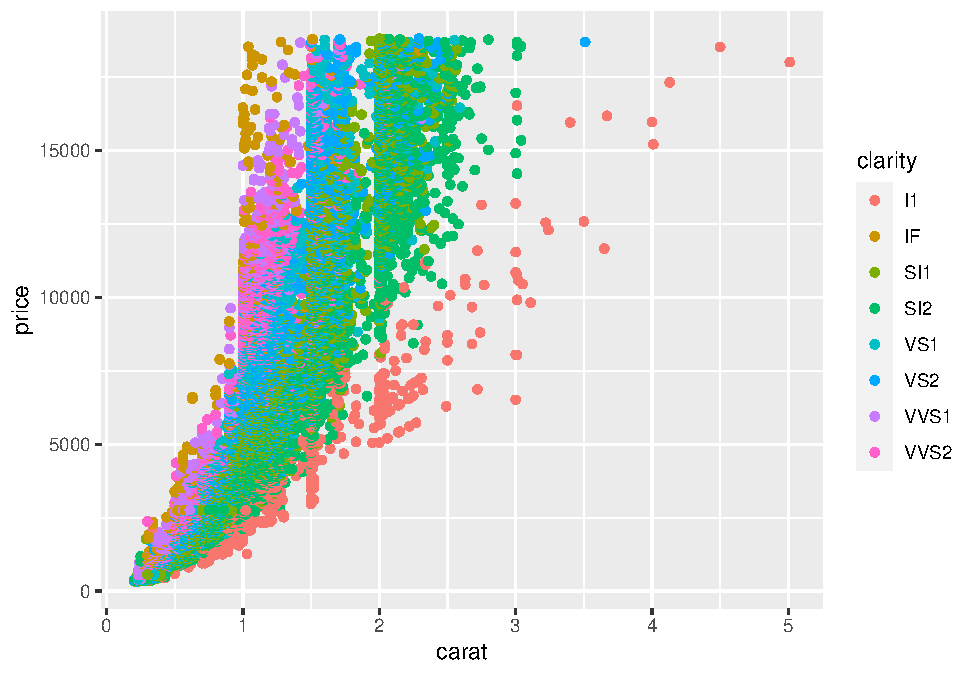
\includegraphics{ENG_792-AVDR_files/figure-latex/Exemplo_1.2-1.pdf}

Vamos nos livrar dos pontos não significativos, aqueles que são \emph{carat} menores que 2.5.

\begin{Shaded}
\begin{Highlighting}[]
\FunctionTok{ggplot}\NormalTok{(}\AttributeTok{data=}\NormalTok{mydata,}
       \FunctionTok{aes}\NormalTok{(}\AttributeTok{x=}\NormalTok{carat, }\AttributeTok{y=}\NormalTok{price, }\AttributeTok{colour=}\NormalTok{clarity))}\SpecialCharTok{+}
\FunctionTok{geom\_point}\NormalTok{(}\AttributeTok{alpha=}\FloatTok{0.1}\NormalTok{) }
\end{Highlighting}
\end{Shaded}

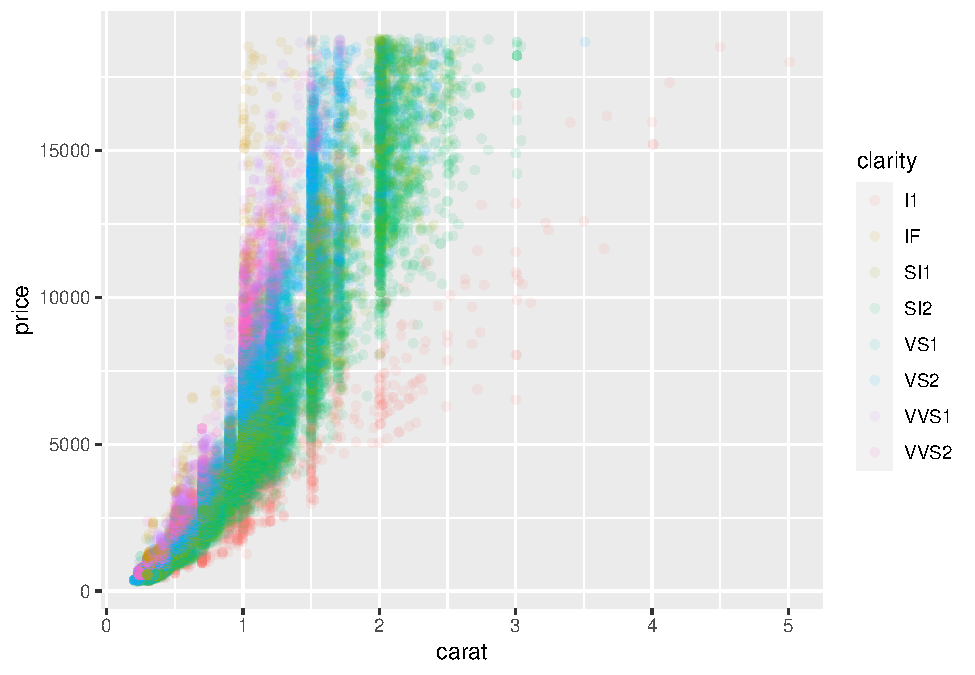
\includegraphics{ENG_792-AVDR_files/figure-latex/Exemplo_1.3-1.pdf}

\textbf{brown} é a melhor claridade, vejam que temos mispricing onde as linhas se cruzam.

\begin{Shaded}
\begin{Highlighting}[]
\FunctionTok{ggplot}\NormalTok{(}\AttributeTok{data=}\NormalTok{mydata[mydata}\SpecialCharTok{$}\NormalTok{carat}\SpecialCharTok{\textless{}}\FloatTok{2.5}\NormalTok{,],}
       \FunctionTok{aes}\NormalTok{(}\AttributeTok{x=}\NormalTok{carat, }\AttributeTok{y=}\NormalTok{price, }\AttributeTok{colour=}\NormalTok{clarity))}\SpecialCharTok{+}
\FunctionTok{geom\_point}\NormalTok{(}\AttributeTok{alpha=}\FloatTok{0.1}\NormalTok{) }\SpecialCharTok{+}
  \FunctionTok{geom\_smooth}\NormalTok{()}
\end{Highlighting}
\end{Shaded}

\begin{verbatim}
## `geom_smooth()` using method = 'gam' and formula 'y ~ s(x, bs = "cs")'
\end{verbatim}

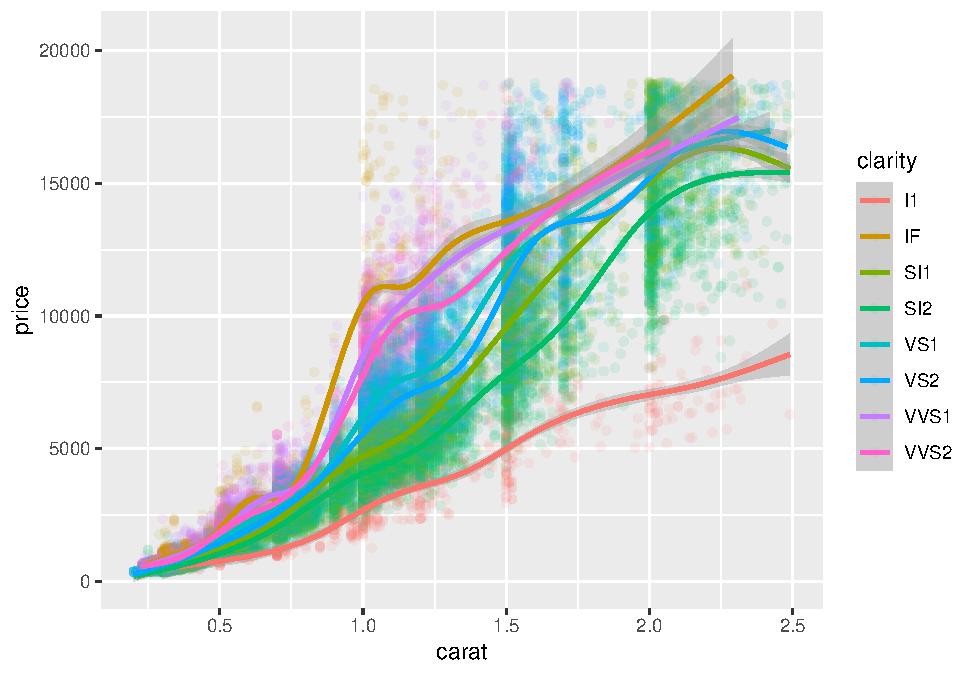
\includegraphics{ENG_792-AVDR_files/figure-latex/Exemplo_1.4-1.pdf}

Executando o código abaixo você produzirá uma Modelo Digital do Terreno em 3D em uma janela \textbf{pop up} do pacote \href{https://www.rayshader.com/}{rayshader}.

\begin{Shaded}
\begin{Highlighting}[]
\FunctionTok{library}\NormalTok{(rayrender)}
\FunctionTok{library}\NormalTok{(rayshader)}
\FunctionTok{library}\NormalTok{(magick)}

\CommentTok{\#Here, I load a map with the raster package.}
\NormalTok{loadzip }\OtherTok{=} \FunctionTok{tempfile}\NormalTok{() }
\FunctionTok{download.file}\NormalTok{(}\StringTok{"https://tylermw.com/data/dem\_01.tif.zip"}\NormalTok{, loadzip)}
\NormalTok{localtif }\OtherTok{=}\NormalTok{ raster}\SpecialCharTok{::}\FunctionTok{raster}\NormalTok{(}\FunctionTok{unzip}\NormalTok{(loadzip, }\StringTok{"dem\_01.tif"}\NormalTok{))}
\FunctionTok{unlink}\NormalTok{(loadzip)}

\CommentTok{\#And convert it to a matrix:}
\NormalTok{elmat }\OtherTok{=} \FunctionTok{raster\_to\_matrix}\NormalTok{(localtif)}

\CommentTok{\#We use another one of rayshader\textquotesingle{}s built{-}in textures:}
\NormalTok{elmat }\SpecialCharTok{\%\textgreater{}\%}
  \FunctionTok{sphere\_shade}\NormalTok{(}\AttributeTok{texture =} \StringTok{"desert"}\NormalTok{) }\SpecialCharTok{\%\textgreater{}\%}
  \FunctionTok{add\_water}\NormalTok{(}\FunctionTok{detect\_water}\NormalTok{(elmat), }\AttributeTok{color =} \StringTok{"desert"}\NormalTok{) }\SpecialCharTok{\%\textgreater{}\%}
  \FunctionTok{plot\_3d}\NormalTok{(elmat, }\AttributeTok{zscale =} \DecValTok{10}\NormalTok{, }\AttributeTok{fov =} \DecValTok{0}\NormalTok{, }\AttributeTok{theta =} \DecValTok{60}\NormalTok{, }\AttributeTok{zoom =} \FloatTok{0.75}\NormalTok{, }\AttributeTok{phi =} \DecValTok{45}\NormalTok{, }\AttributeTok{windowsize =} \FunctionTok{c}\NormalTok{(}\DecValTok{1000}\NormalTok{, }\DecValTok{800}\NormalTok{))}
\end{Highlighting}
\end{Shaded}

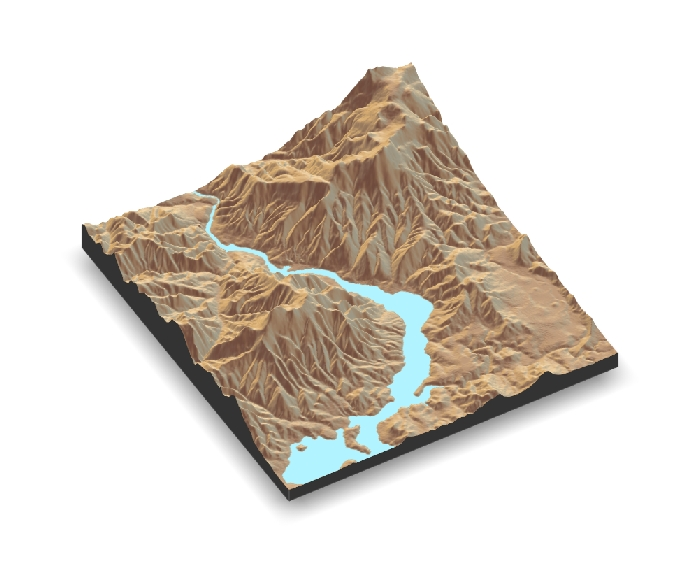
\includegraphics{J:/ENG 792/ENG_792-AVDR/ENG.792-AVDR/Cap_1_rayshader.jpeg}

Agora vamos adicionar mais algumas infromações como escala e Norte.

\begin{Shaded}
\begin{Highlighting}[]
\FunctionTok{render\_scalebar}\NormalTok{(}\AttributeTok{limits=}\FunctionTok{c}\NormalTok{(}\DecValTok{0}\NormalTok{, }\DecValTok{5}\NormalTok{, }\DecValTok{10}\NormalTok{),}\AttributeTok{label\_unit =} \StringTok{"km"}\NormalTok{,}\AttributeTok{position =} \StringTok{"W"}\NormalTok{, }\AttributeTok{y=}\DecValTok{50}\NormalTok{,}\AttributeTok{scale\_length =} \FunctionTok{c}\NormalTok{(}\FloatTok{0.33}\NormalTok{,}\DecValTok{1}\NormalTok{))}

\FunctionTok{render\_compass}\NormalTok{(}\AttributeTok{position =} \StringTok{"E"}\NormalTok{)}
\FunctionTok{Sys.sleep}\NormalTok{(}\FloatTok{0.2}\NormalTok{)}
\FunctionTok{render\_highquality}\NormalTok{(}\AttributeTok{samples=}\DecValTok{200}\NormalTok{, }\AttributeTok{scale\_text\_size =} \DecValTok{24}\NormalTok{,}\AttributeTok{clear=}\ConstantTok{TRUE}\NormalTok{)}
\end{Highlighting}
\end{Shaded}

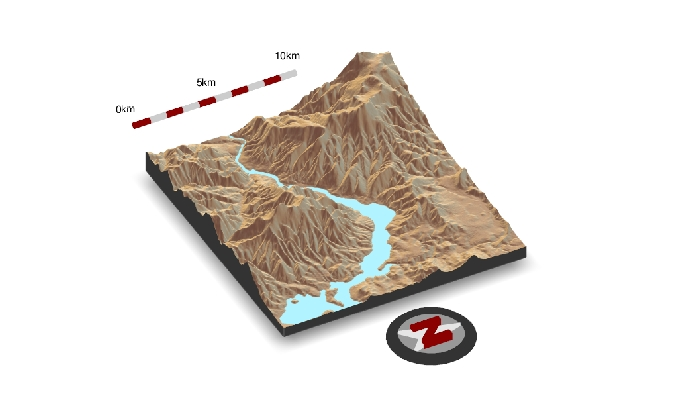
\includegraphics[width=1.2\textwidth,height=1.2\textheight]{J:/ENG 792/ENG_792-AVDR/ENG.792-AVDR/Cap_1_rayshader2.jpeg}

\hypertarget{como-r-funciona}{%
\section{Como R funciona}\label{como-r-funciona}}

Diferentemente de outras linguagens, todos os comandos escritos são diretamente executados, desta forma o R não precisa de um compilador para executar os comandos como Fortran. Por isso, torna-se uma linguagem muito mais amigável e acessível para não programadores.

A linguagem é muito intuitiva (quase uma sintaxe lógica). Por exemplo uma regressão linear pode ser executada como \emph{lm(x\textasciitilde y)} ( \emph{\emph{lm}} vem de \emph{\emph{linear model}}). Como no exemplo do modelo linear acima, sempre que formos executar um comando temos que seguir da seguinte forma \emph{\emph{função(dados e demais ajustes ou parâmetros)}}, ou seja chame a função e coloque o resto dentro de parênteses.

Como dito anteriormente em aula, tudo que é executado pelo R fica armazenado na memória ativa (RAM) do computador na forma de objetos que possuem um nome. Os objetos, que variam em tipos e estruturas, podem ser funções criadas pelo próprio usuário, dados criados ou importados de uma memória, expressões e etc. Antes de entrarmos em detalhes sobre funções ou expressões, vamos nos ater aos objetos enquanto tipo na sequência suas estruturas.

Dica de livro de cabeceira sobre R \citet{melloandpeternelli2013}.

\hypertarget{tipos-de-objetos}{%
\subsection{Tipos de objetos}\label{tipos-de-objetos}}

Os objetos no R podem ser do tipo \emph{lógico}, \emph{inteiro}, \emph{simples}, \emph{dupla}, \emph{complexo}, \emph{função} ou \emph{caractere}.

\begin{tabular}{l|l|l}
\hline
mode() & Armazenamento & Exemplo\\
\hline
logical & lógico & TRUE or FALSE\\
\hline
numeric & inteiro, simples ou dupla & Números 1, 3.14, 2e-308 etc\\
\hline
complex & complexo & 3+2i\\
\hline
function & função & Soma<-function(...)\\
\hline
name & caractere & média\\
\hline
\end{tabular}

\textbf{Tabela 1:} Tipos de modos para objetos no R.

\begin{Shaded}
\begin{Highlighting}[]
\CommentTok{\#logical}
\NormalTok{q1 }\OtherTok{\textless{}{-}}\NormalTok{T}
\FunctionTok{mode}\NormalTok{(q1);}\FunctionTok{typeof}\NormalTok{(q1)}
\end{Highlighting}
\end{Shaded}

\begin{verbatim}
## [1] "logical"
\end{verbatim}

\begin{verbatim}
## [1] "logical"
\end{verbatim}

\begin{Shaded}
\begin{Highlighting}[]
\NormalTok{q2 }\OtherTok{\textless{}{-}} \ConstantTok{FALSE} \CommentTok{\#pode ser a palavra toda mas em maiúsculas }
\FunctionTok{mode}\NormalTok{(q2);}\FunctionTok{typeof}\NormalTok{(q2)}
\end{Highlighting}
\end{Shaded}

\begin{verbatim}
## [1] "logical"
\end{verbatim}

\begin{verbatim}
## [1] "logical"
\end{verbatim}

\begin{Shaded}
\begin{Highlighting}[]
\CommentTok{\#integer}
\NormalTok{x}\OtherTok{\textless{}{-}}\NormalTok{2L }\CommentTok{\#L garante que 2 será integer}
\FunctionTok{mode}\NormalTok{(x);}\FunctionTok{typeof}\NormalTok{(x)}
\end{Highlighting}
\end{Shaded}

\begin{verbatim}
## [1] "numeric"
\end{verbatim}

\begin{verbatim}
## [1] "integer"
\end{verbatim}

\begin{Shaded}
\begin{Highlighting}[]
\CommentTok{\#double}
\NormalTok{y}\OtherTok{\textless{}{-}}\FloatTok{2.5}
\FunctionTok{mode}\NormalTok{(y);}\FunctionTok{typeof}\NormalTok{(y)}
\end{Highlighting}
\end{Shaded}

\begin{verbatim}
## [1] "numeric"
\end{verbatim}

\begin{verbatim}
## [1] "double"
\end{verbatim}

\begin{Shaded}
\begin{Highlighting}[]
\CommentTok{\#Complex}
\NormalTok{z}\OtherTok{\textless{}{-}}\DecValTok{3}\SpecialCharTok{+}\NormalTok{2i}
\FunctionTok{mode}\NormalTok{(z);}\FunctionTok{typeof}\NormalTok{(z)}
\end{Highlighting}
\end{Shaded}

\begin{verbatim}
## [1] "complex"
\end{verbatim}

\begin{verbatim}
## [1] "complex"
\end{verbatim}

\begin{Shaded}
\begin{Highlighting}[]
\CommentTok{\#function}
\NormalTok{Soma}\OtherTok{\textless{}{-}}\ControlFlowTok{function}\NormalTok{(x,y)\{}
\NormalTok{  x}\SpecialCharTok{+}\NormalTok{y}
\NormalTok{\}}
\FunctionTok{mode}\NormalTok{(Soma);}\FunctionTok{typeof}\NormalTok{(Soma)}
\end{Highlighting}
\end{Shaded}

\begin{verbatim}
## [1] "function"
\end{verbatim}

\begin{verbatim}
## [1] "closure"
\end{verbatim}

\begin{Shaded}
\begin{Highlighting}[]
\CommentTok{\#Character}
\NormalTok{a }\OtherTok{\textless{}{-}}\StringTok{"h"} \CommentTok{\#Para colocar uma letra em uma variável é preciso colocar entre "")}
\FunctionTok{mode}\NormalTok{(a);}\FunctionTok{typeof}\NormalTok{(a)}
\end{Highlighting}
\end{Shaded}

\begin{verbatim}
## [1] "character"
\end{verbatim}

\begin{verbatim}
## [1] "character"
\end{verbatim}

\begin{Shaded}
\begin{Highlighting}[]
\NormalTok{média}\OtherTok{\textless{}{-}}\StringTok{"média"}
\FunctionTok{mode}\NormalTok{(a);}\FunctionTok{typeof}\NormalTok{(a)}
\end{Highlighting}
\end{Shaded}

\begin{verbatim}
## [1] "character"
\end{verbatim}

\begin{verbatim}
## [1] "character"
\end{verbatim}

Saber as diferenças entre os diversos objetos é importante para uma exploração mais adequada dos dados, utilização eficiente de funções ou operações lógicas, artiméticas, estatísticas e etc.

Veja que no caso acima em \emph{integer} (x \textless- 2L) optamos por adicionar ``L'' após o número 2, pois o R por padrão decide onde e como aloca/aloja/armazena um operador. A informação será preferencialmente salva como \emph{double} e isso faz sentido caso você queira mais adiante realizar operações com números decimais ou realizar operações que resultem em números decimais.

No entanto, caso queira saber que tipo de dado está manipulado você pode ``perguntar'' utilizando \emph{is.} seguido da designação do tipo de dados quer testar ( \emph{integer}, \emph{numeric}, \emph{double} e etc) e teremos uma resposta lógica.

\begin{Shaded}
\begin{Highlighting}[]
\FunctionTok{is.double}\NormalTok{(x) }
\end{Highlighting}
\end{Shaded}

\begin{verbatim}
## [1] FALSE
\end{verbatim}

Caso você deseje que sua variável seja de um tipo específico, você pode transformá-la utilizando \emph{as.} seguido da designação desejada ( \emph{integer}, \emph{numeric}, \emph{double} e etc).

\begin{Shaded}
\begin{Highlighting}[]
\NormalTok{x}\OtherTok{\textless{}{-}}\FunctionTok{as.double}\NormalTok{(x)}
\FunctionTok{is.double}\NormalTok{(x)}
\end{Highlighting}
\end{Shaded}

\begin{verbatim}
## [1] TRUE
\end{verbatim}

Cada tipo de dado é associado com um teste e uma função de conversão conforme a tabela 2.

\begin{tabular}{l|l|l}
\hline
Tipo & Teste & Função de conversão\\
\hline
character & is.character & as.character\\
\hline
complex & is.complex & as.complex\\
\hline
double & is.double & as.double\\
\hline
expression & is.expression & as.expression\\
\hline
integer & is.integer & as.integer\\
\hline
list & is.list & as.list\\
\hline
logical & is.logical & as.logical\\
\hline
numeric & is.numeric & as.numeric\\
\hline
single & is.single & as.single\\
\hline
raw & is.raw & as.raw\\
\hline
Date & is.Date & as.Date\\
\hline
\end{tabular}

\textbf{Tabela 2:} Tipos de dados, teste e modos de conversão.

\hypertarget{estrutura-do-objetos}{%
\subsection{Estrutura do objetos}\label{estrutura-do-objetos}}

As informações armazenadas em objetos no R podem ser organizadas em diferentes estruturas.

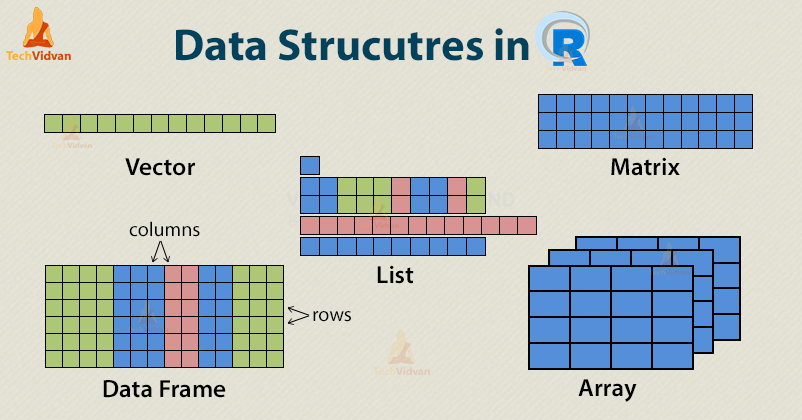
\includegraphics[width=0.5\textwidth,height=0.5\textheight]{J:/ENG 792/ENG_792-AVDR/ENG.792-AVDR/Cap_1_R_data_strucutres.jpg}

\textbf{Figura 1:} Estrutura de dados no R. Fonte: \href{https://techvidvan.com/tutorials/r-data-structures/}{techvidvan}

\begin{tabular}{l|l|l}
\hline
Objeto & modes & descrição\\
\hline
vector & numeric, character, complex ou logical & Com um ou  mais elementos\\
\hline
factor & numeric ou character & Vetor que representa dados categóricos\\
\hline
matriz & numeric, character, complex ou logical & Um array de duas dimensões\\
\hline
array & numeric, character, complex ou logical & Pode conter um, duas ou mais dimensões\\
\hline
data frame & numeric, character, complex ou logical & Um array de duas dimenões que permite colunas de diferentes tipos dem mesmo objeto\\
\hline
list & numeric, character, complex, logical, function, expression, ... & Objeto que permite combinar diferentes estruturtas de dados num único objeto\\
\hline
\end{tabular}

\textbf{Tabela 3:} Características dos tipos de objetos.

\hypertarget{vetores-vectors}{%
\subsubsection{\texorpdfstring{Vetores (\emph{Vectors})}{Vetores (Vectors)}}\label{vetores-vectors}}

Vetores são os tipos de objetos mais comuns no R. Um vetor é composto de uma informação ou uma séries de informações ( \emph{arrays} ) unidimensionais que podem conter informaçõs numéricas, caracteres ou dados lógicos.

Mesmo quando digitamos apoenas um único elemento ele se torna um vetor de comprimento um (1).

\emph{Vetores com Apenas 1 elemento}

\begin{Shaded}
\begin{Highlighting}[]
\NormalTok{esquerdo}\OtherTok{\textless{}{-}}\NormalTok{(}\StringTok{"direito"}\NormalTok{) }\CommentTok{\# O objeto "esquerdo" recebe a palavra "direito"}
\NormalTok{esquerdo }\CommentTok{\#execute o arquivo e veja seu conteúdo}
\end{Highlighting}
\end{Shaded}

\begin{verbatim}
## [1] "direito"
\end{verbatim}

\begin{Shaded}
\begin{Highlighting}[]
\NormalTok{direito}\OtherTok{=}\FunctionTok{c}\NormalTok{(}\StringTok{"esquerdo"}\NormalTok{) }\CommentTok{\#Outra maneira de criar objeto  }
\FunctionTok{print}\NormalTok{(direito) }\CommentTok{\#Outra forma de executar o conteúdo}
\end{Highlighting}
\end{Shaded}

\begin{verbatim}
## [1] "esquerdo"
\end{verbatim}

\begin{Shaded}
\begin{Highlighting}[]
\NormalTok{b}\OtherTok{=}\NormalTok{(}\DecValTok{10}\NormalTok{) }\CommentTok{\# O objeto "b" recebe o número 10}
\NormalTok{b}
\end{Highlighting}
\end{Shaded}

\begin{verbatim}
## [1] 10
\end{verbatim}

\begin{Shaded}
\begin{Highlighting}[]
\NormalTok{(}\FloatTok{15.23}\NormalTok{)}\OtherTok{{-}\textgreater{}}\NormalTok{c }\CommentTok{\# O objeto "c" recebe o número 15.23}
\NormalTok{c}
\end{Highlighting}
\end{Shaded}

\begin{verbatim}
## [1] 15.23
\end{verbatim}

Vetores com múltiplos elementos

\begin{Shaded}
\begin{Highlighting}[]
\NormalTok{d}\OtherTok{\textless{}{-}}\NormalTok{(}\DecValTok{0}\SpecialCharTok{:}\DecValTok{10}\NormalTok{) }\CommentTok{\# Criando uma sequência de 0 até 10}
\NormalTok{d}
\end{Highlighting}
\end{Shaded}

\begin{verbatim}
##  [1]  0  1  2  3  4  5  6  7  8  9 10
\end{verbatim}

\begin{Shaded}
\begin{Highlighting}[]
\NormalTok{e}\OtherTok{\textless{}{-}}\FloatTok{10.5}\SpecialCharTok{:}\FloatTok{20.5} \CommentTok{\# criando uma sequência de 10.5 até 20.5}
\NormalTok{e}
\end{Highlighting}
\end{Shaded}

\begin{verbatim}
##  [1] 10.5 11.5 12.5 13.5 14.5 15.5 16.5 17.5 18.5 19.5 20.5
\end{verbatim}

\begin{Shaded}
\begin{Highlighting}[]
\NormalTok{f}\OtherTok{\textless{}{-}}\NormalTok{(}\FloatTok{10.6}\SpecialCharTok{:}\FloatTok{20.3}\NormalTok{) }\CommentTok{\# O último elemento é descartado por nãos e encaixar na sequência}
\NormalTok{f}
\end{Highlighting}
\end{Shaded}

\begin{verbatim}
##  [1] 10.6 11.6 12.6 13.6 14.6 15.6 16.6 17.6 18.6 19.6
\end{verbatim}

Podemos utilizar também a função \emph{seq} para gerar uma sequêncaio de dados

\emph{\emph{seq(from = 1, to = 1, by = ((to - from)/(length.out - 1)),length.out = NULL, along.with = NULL, \ldots)}}

\begin{Shaded}
\begin{Highlighting}[]
\NormalTok{g}\OtherTok{\textless{}{-}}\FunctionTok{seq}\NormalTok{(}\DecValTok{0}\NormalTok{,}\DecValTok{10}\NormalTok{,}\FloatTok{0.5}\NormalTok{) }\CommentTok{\# O objeto "g" recebe a sequência de 0 até 10 a cada 0.5}
\NormalTok{g}
\end{Highlighting}
\end{Shaded}

\begin{verbatim}
##  [1]  0.0  0.5  1.0  1.5  2.0  2.5  3.0  3.5  4.0  4.5  5.0  5.5  6.0  6.5  7.0
## [16]  7.5  8.0  8.5  9.0  9.5 10.0
\end{verbatim}

\begin{Shaded}
\begin{Highlighting}[]
\NormalTok{h}\OtherTok{\textless{}{-}}\FunctionTok{seq}\NormalTok{(}\AttributeTok{from=}\DecValTok{10}\NormalTok{,}\AttributeTok{to=}\DecValTok{20}\NormalTok{,}\AttributeTok{length.out=}\DecValTok{50}\NormalTok{) }\CommentTok{\# O objeto "h" recebe a sequência de 0 até 10 que é do compriumento 50, ou seja, há 50 número de 10 até 20}
\NormalTok{h}
\end{Highlighting}
\end{Shaded}

\begin{verbatim}
##  [1] 10.00000 10.20408 10.40816 10.61224 10.81633 11.02041 11.22449 11.42857
##  [9] 11.63265 11.83673 12.04082 12.24490 12.44898 12.65306 12.85714 13.06122
## [17] 13.26531 13.46939 13.67347 13.87755 14.08163 14.28571 14.48980 14.69388
## [25] 14.89796 15.10204 15.30612 15.51020 15.71429 15.91837 16.12245 16.32653
## [33] 16.53061 16.73469 16.93878 17.14286 17.34694 17.55102 17.75510 17.95918
## [41] 18.16327 18.36735 18.57143 18.77551 18.97959 19.18367 19.38776 19.59184
## [49] 19.79592 20.00000
\end{verbatim}

Experimente também a função \emph{rep()}

\emph{\emph{rep(x, times = 1, length.out = NA, each = 1)}}

\begin{Shaded}
\begin{Highlighting}[]
\NormalTok{i}\OtherTok{\textless{}{-}}\FunctionTok{rep}\NormalTok{(}\DecValTok{0}\NormalTok{,}\DecValTok{10}\NormalTok{) }\CommentTok{\# O objeto "i" recebe 10 números 1}
\NormalTok{i}
\end{Highlighting}
\end{Shaded}

\begin{verbatim}
##  [1] 0 0 0 0 0 0 0 0 0 0
\end{verbatim}

\begin{Shaded}
\begin{Highlighting}[]
\NormalTok{j}\OtherTok{\textless{}{-}}\FunctionTok{rep}\NormalTok{(}\FunctionTok{c}\NormalTok{(}\DecValTok{1}\SpecialCharTok{:}\DecValTok{3}\NormalTok{),}\DecValTok{10}\NormalTok{) }\CommentTok{\# O objeto "j" recebe 10 vezes a sequência 1, 2 e 3}
\NormalTok{j}
\end{Highlighting}
\end{Shaded}

\begin{verbatim}
##  [1] 1 2 3 1 2 3 1 2 3 1 2 3 1 2 3 1 2 3 1 2 3 1 2 3 1 2 3 1 2 3
\end{verbatim}

\textbf{Um Vetor só pode conter informações de um único tipo}

\begin{Shaded}
\begin{Highlighting}[]
\NormalTok{k}\OtherTok{\textless{}{-}}\FunctionTok{c}\NormalTok{(}\DecValTok{0}\NormalTok{,}\DecValTok{1}\NormalTok{,}\DecValTok{2}\NormalTok{,}\DecValTok{3}\NormalTok{,}\DecValTok{4}\NormalTok{, }\StringTok{"A"}\NormalTok{) }\CommentTok{\# O objeto "k" é do tipo character por causa de "A"}
\FunctionTok{typeof}\NormalTok{(k);}\FunctionTok{mode}\NormalTok{(k)}
\end{Highlighting}
\end{Shaded}

\begin{verbatim}
## [1] "character"
\end{verbatim}

\begin{verbatim}
## [1] "character"
\end{verbatim}

\begin{Shaded}
\begin{Highlighting}[]
\NormalTok{l}\OtherTok{\textless{}{-}}\FunctionTok{c}\NormalTok{(}\DecValTok{0}\NormalTok{,}\DecValTok{1}\NormalTok{,}\DecValTok{2}\NormalTok{,}\DecValTok{3}\NormalTok{,}\DecValTok{4}\NormalTok{) }\CommentTok{\# O objeto "l" é do tipo numérico}
\FunctionTok{typeof}\NormalTok{(l);}\FunctionTok{mode}\NormalTok{(l)}
\end{Highlighting}
\end{Shaded}

\begin{verbatim}
## [1] "double"
\end{verbatim}

\begin{verbatim}
## [1] "numeric"
\end{verbatim}

\hypertarget{fatores-factors}{%
\subsubsection{\texorpdfstring{Fatores (\emph{Factors})}{Fatores (Factors)}}\label{fatores-factors}}

Os fatores são vetores em que os elementos pertencem a uma ou mais categorias temáticas.
As variáveis aleatórias podem ser divididas em contínuas e categóricas.

\begin{itemize}
\tightlist
\item
  As contínuas podem ser medidas nas escalas: relacional e intervalar.
\item
  As categóricas nas escalas: nominal e ordinal.
\end{itemize}

No R, as variáveis categóricas medidas nas escalas nominal e ordinal são chamados fatores.
A função \emph{factor()} armazenas os valores categóricos como um vetor de inteiros {[}1..k{]} e um vetor interno de \emph{strings} referentes ao nomes.
\emph{Em outras palavras, um \textbf{factor} é um \textbf{vetor} objeto usado para especificar uma classsificação discreta (agrupamento) dos componentes de outros vetores de mesmo tamanho.}

\emph{\emph{factor(x = character(), levels, labels = levels,exclude = NA, ordered = is.ordered(x), nmax = NA)}}

ou

\emph{\emph{gl(n, k, length = n X k, labels = seq\_len(n), ordered = FALSE)}}

\begin{Shaded}
\begin{Highlighting}[]
\NormalTok{m}\OtherTok{\textless{}{-}}\FunctionTok{factor}\NormalTok{(}\FunctionTok{c}\NormalTok{(}\StringTok{"H"}\NormalTok{,}\StringTok{"H"}\NormalTok{,}\StringTok{"H"}\NormalTok{,}\StringTok{"M"}\NormalTok{,}\StringTok{"M"}\NormalTok{)) }\CommentTok{\# O objeto "k" recebe 3 H\textquotesingle{}s e 2 M\textquotesingle{}s}
\NormalTok{m}
\end{Highlighting}
\end{Shaded}

\begin{verbatim}
## [1] H H H M M
## Levels: H M
\end{verbatim}

\begin{Shaded}
\begin{Highlighting}[]
\FunctionTok{as.integer}\NormalTok{(m)}
\end{Highlighting}
\end{Shaded}

\begin{verbatim}
## [1] 1 1 1 2 2
\end{verbatim}

\begin{Shaded}
\begin{Highlighting}[]
\NormalTok{n}\OtherTok{\textless{}{-}}\FunctionTok{gl}\NormalTok{(}\AttributeTok{n=}\DecValTok{2}\NormalTok{,}\AttributeTok{k=}\DecValTok{3}\NormalTok{,}\AttributeTok{labels=}\FunctionTok{c}\NormalTok{(}\StringTok{"M"}\NormalTok{,}\StringTok{"F"}\NormalTok{)) }
\NormalTok{n}
\end{Highlighting}
\end{Shaded}

\begin{verbatim}
## [1] M M M F F F
## Levels: M F
\end{verbatim}

Podemos verificar os níveis de um fator usando o comando \emph{levels()}.

\begin{Shaded}
\begin{Highlighting}[]
\FunctionTok{levels}\NormalTok{(m)}
\end{Highlighting}
\end{Shaded}

\begin{verbatim}
## [1] "H" "M"
\end{verbatim}

\begin{Shaded}
\begin{Highlighting}[]
\FunctionTok{levels}\NormalTok{(n)}
\end{Highlighting}
\end{Shaded}

\begin{verbatim}
## [1] "M" "F"
\end{verbatim}

\hypertarget{matriz-matrix}{%
\subsubsection{\texorpdfstring{Matriz (\emph{Matrix})}{Matriz (Matrix)}}\label{matriz-matrix}}

É o tipo de dado mais comum que encontramos do dia a dia. A maioria dos dados que analisamos estão organizados em matrizes que são dados combinados em 2 dimensões (linas e colunas).
Existem várias maneiras de criar uma matriz como utilizando o comando \emph{matrix()}.

\emph{\emph{matrix(data = NA, nrow = 1, ncol = 1, byrow = FALSE,dimnames = NULL)}}

Assim como os vetores, as matrizes só aceitam dados do mesmo tipo.

\begin{Shaded}
\begin{Highlighting}[]
\NormalTok{o}\OtherTok{\textless{}{-}}\DecValTok{1}\SpecialCharTok{:}\DecValTok{10} \CommentTok{\# cria um vetor de 1 a 10}
\NormalTok{o\_matriz1}\OtherTok{\textless{}{-}}\FunctionTok{matrix}\NormalTok{(o,}\AttributeTok{ncol=}\DecValTok{5}\NormalTok{)}\CommentTok{\# Organiza o vetor 0 e 5 colunas}
\NormalTok{o\_matriz1}
\end{Highlighting}
\end{Shaded}

\begin{verbatim}
##      [,1] [,2] [,3] [,4] [,5]
## [1,]    1    3    5    7    9
## [2,]    2    4    6    8   10
\end{verbatim}

\begin{Shaded}
\begin{Highlighting}[]
\NormalTok{o\_matriz2}\OtherTok{\textless{}{-}}\FunctionTok{matrix}\NormalTok{(o,}\AttributeTok{nrow=}\DecValTok{5}\NormalTok{)}\CommentTok{\# Organiza o vetor 0 e 5 linhas}
\NormalTok{o\_matriz2}
\end{Highlighting}
\end{Shaded}

\begin{verbatim}
##      [,1] [,2]
## [1,]    1    6
## [2,]    2    7
## [3,]    3    8
## [4,]    4    9
## [5,]    5   10
\end{verbatim}

Podemos utilizar também o argumento \emph{byrow=}, que, diferente do exemplo acima, preenchem as tabelas por linhas.

\begin{Shaded}
\begin{Highlighting}[]
\NormalTok{p}\OtherTok{\textless{}{-}}\DecValTok{1}\SpecialCharTok{:}\DecValTok{10} \CommentTok{\# cria um vetor de 1 a 10}
\NormalTok{p\_matriz1}\OtherTok{\textless{}{-}}\FunctionTok{matrix}\NormalTok{(o,}\AttributeTok{nrow=}\DecValTok{5}\NormalTok{,}\AttributeTok{byrow=}\NormalTok{T)}\CommentTok{\# Organiza o vetor 0 e 5 colunas}
\NormalTok{p\_matriz1; o\_matriz2 }\CommentTok{\# compare os 2 modos}
\end{Highlighting}
\end{Shaded}

\begin{verbatim}
##      [,1] [,2]
## [1,]    1    2
## [2,]    3    4
## [3,]    5    6
## [4,]    7    8
## [5,]    9   10
\end{verbatim}

\begin{verbatim}
##      [,1] [,2]
## [1,]    1    6
## [2,]    2    7
## [3,]    3    8
## [4,]    4    9
## [5,]    5   10
\end{verbatim}

As dimensões de uma matriz pode ser acessado através do comando \emph{dim()}:

\begin{Shaded}
\begin{Highlighting}[]
\FunctionTok{dim}\NormalTok{(o\_matriz1);}\FunctionTok{dim}\NormalTok{(o\_matriz2) }\CommentTok{\# Leia o o resultado como linha e coluna}
\end{Highlighting}
\end{Shaded}

\begin{verbatim}
## [1] 2 5
\end{verbatim}

\begin{verbatim}
## [1] 5 2
\end{verbatim}

Também é interessante usar o comando \emph{summary()}.

\begin{Shaded}
\begin{Highlighting}[]
\FunctionTok{summary}\NormalTok{(o\_matriz1);}\FunctionTok{summary}\NormalTok{(o\_matriz2) }\CommentTok{\# Mostra informações por coluna}
\end{Highlighting}
\end{Shaded}

\begin{verbatim}
##        V1             V2             V3             V4             V5       
##  Min.   :1.00   Min.   :3.00   Min.   :5.00   Min.   :7.00   Min.   : 9.00  
##  1st Qu.:1.25   1st Qu.:3.25   1st Qu.:5.25   1st Qu.:7.25   1st Qu.: 9.25  
##  Median :1.50   Median :3.50   Median :5.50   Median :7.50   Median : 9.50  
##  Mean   :1.50   Mean   :3.50   Mean   :5.50   Mean   :7.50   Mean   : 9.50  
##  3rd Qu.:1.75   3rd Qu.:3.75   3rd Qu.:5.75   3rd Qu.:7.75   3rd Qu.: 9.75  
##  Max.   :2.00   Max.   :4.00   Max.   :6.00   Max.   :8.00   Max.   :10.00
\end{verbatim}

\begin{verbatim}
##        V1          V2    
##  Min.   :1   Min.   : 6  
##  1st Qu.:2   1st Qu.: 7  
##  Median :3   Median : 8  
##  Mean   :3   Mean   : 8  
##  3rd Qu.:4   3rd Qu.: 9  
##  Max.   :5   Max.   :10
\end{verbatim}

Outras formas de contruir matrizes é juntando objetos existentes através dos comandos \emph{cbind()} e \emph{rbind()} que contacatenam objetos por colunas e linhas, respectivamente.

Vamos juntar as matrizes já criadas.

\begin{Shaded}
\begin{Highlighting}[]
\NormalTok{o\_matriz3}\OtherTok{\textless{}{-}}\FunctionTok{rbind}\NormalTok{(o\_matriz1,o\_matriz1) }\CommentTok{\# concatena por linhas (r)}
\NormalTok{o\_matriz3}
\end{Highlighting}
\end{Shaded}

\begin{verbatim}
##      [,1] [,2] [,3] [,4] [,5]
## [1,]    1    3    5    7    9
## [2,]    2    4    6    8   10
## [3,]    1    3    5    7    9
## [4,]    2    4    6    8   10
\end{verbatim}

\begin{Shaded}
\begin{Highlighting}[]
\NormalTok{o\_matriz4}\OtherTok{\textless{}{-}}\FunctionTok{rbind}\NormalTok{(o\_matriz2,o\_matriz2) }\CommentTok{\# concatena por colunas (c)}
\NormalTok{o\_matriz4}
\end{Highlighting}
\end{Shaded}

\begin{verbatim}
##       [,1] [,2]
##  [1,]    1    6
##  [2,]    2    7
##  [3,]    3    8
##  [4,]    4    9
##  [5,]    5   10
##  [6,]    1    6
##  [7,]    2    7
##  [8,]    3    8
##  [9,]    4    9
## [10,]    5   10
\end{verbatim}

\hypertarget{array}{%
\subsubsection{Array}\label{array}}

O array é um conjunto de matrizes ou vetores que podem ter qualquer número de dimensões. Estas dimensões podem receber nomes.
Podemos criar \emph{arrays} atribuindo dimensçoes a um vetor com o comando \emph{dim()} ou usando \emph{array()}.

\emph{\emph{array(data = NA, dim = length(data), dimnames = NULL)}}

\begin{Shaded}
\begin{Highlighting}[]
\NormalTok{q\_array}\OtherTok{\textless{}{-}}\DecValTok{1}\SpecialCharTok{:}\DecValTok{12} \CommentTok{\# cria um vetor}
\FunctionTok{dim}\NormalTok{(q\_array)}\OtherTok{\textless{}{-}}\FunctionTok{c}\NormalTok{(}\DecValTok{2}\NormalTok{,}\DecValTok{3}\NormalTok{,}\DecValTok{2}\NormalTok{) }\CommentTok{\# atribuindo 3 dimensões a q\_array}
\NormalTok{q\_array}
\end{Highlighting}
\end{Shaded}

\begin{verbatim}
## , , 1
## 
##      [,1] [,2] [,3]
## [1,]    1    3    5
## [2,]    2    4    6
## 
## , , 2
## 
##      [,1] [,2] [,3]
## [1,]    7    9   11
## [2,]    8   10   12
\end{verbatim}

\begin{Shaded}
\begin{Highlighting}[]
\NormalTok{r\_array}\OtherTok{\textless{}{-}}\FunctionTok{array}\NormalTok{(}\DecValTok{1}\SpecialCharTok{:}\DecValTok{12}\NormalTok{,}\FunctionTok{c}\NormalTok{(}\DecValTok{2}\NormalTok{,}\DecValTok{3}\NormalTok{,}\DecValTok{2}\NormalTok{)) }\CommentTok{\# cria um array de 3 dimensões}
\NormalTok{r\_array}
\end{Highlighting}
\end{Shaded}

\begin{verbatim}
## , , 1
## 
##      [,1] [,2] [,3]
## [1,]    1    3    5
## [2,]    2    4    6
## 
## , , 2
## 
##      [,1] [,2] [,3]
## [1,]    7    9   11
## [2,]    8   10   12
\end{verbatim}

\hypertarget{data-frame}{%
\subsubsection{Data Frame}\label{data-frame}}

Tão comum quanto a matriz, o data frame também um modo bidimensional de organização dos dados (linhas e colunas) que, diferentemente da matriz, permite objetos de tipos diferentes (character, numeric, logical e etc)sejam armazenados.
Normalmente, nos data frames temos nas linhas as observações e nas colunas temos as variáveis.
No entanto, é importante que cada coluna tenha o mesmo tamanho.

\emph{\emph{data.frame(\ldots, row.names = NULL, check.rows = FALSE,check.names = TRUE, fix.empty.names = TRUE,stringsAsFactors = default.stringsAsFactors())}}

\begin{tabular}{l|l|l|l|l}
\hline
Nome & Matrícula & Curso & Nivel.de.R & Nível.Pós\\
\hline
Alberto Domingos Macamo & 0 & Meteorologia Aplicada & NA & Mestrado\\
\hline
Ana Luiza Melo Rodrigues & 98075 & Engenharia Agrícola & 0 & Doutorado\\
\hline
Arieta Carla Gualandi Leal & 88695 & Nutrição & 0 & Doutorado\\
\hline
Caio Henrique Patrício Pagani & 104129 & Engenharia Agrícola & 2 & Doutorado\\
\hline
Carla Larissa Fonseca da Silva & 104731 & Engenharia Agrícola & 3 & Mestrado\\
\hline
Conrado Trigo de Moraes & 104589 & Zootecnia & 1 & Doutorado\\
\hline
Diego Bispo dos Santos Farias & 0 & Engenharia Agrícola & NA & Doutorado\\
\hline
Eloy Junior Rezende & 104599 & Zootecnia & 0 & Mestrado\\
\hline
Fernanda Gonçalves Borges & 104162 & Engenharia Agrícola & 2 & Mestrado\\
\hline
Flávio Dayrell Gontijo & 101417 & Botânica & 4 & Mestrado\\
\hline
Francilene Maria Azevedo & 74843 & Ciência da Nutrição & 1 & Doutorado\\
\hline
Lorena Moreira Lara & 74038 & Fitotecnia (melhoramento) & 5 & Doutorado\\
\hline
Luana Caldeira Fonseca Coutinho & 81919 & Biologia & 1 & Mestrado\\
\hline
Marconi Martins Cunha & 70859 & Engenharia Civil & 3 & Doutorado\\
\hline
Mathias Viana Vicari & 0 & Não informado & NA & Nâo informado\\
\hline
Mayara Oliveira Rocha & 104557 & Engenharia Agrícola & 1 & Doutorado\\
\hline
Michel Henriques de Souza & 74102 & Genética e Melhoramento & 5 & Doutorado\\
\hline
Moana Teixeira Rothe-Neves & 104660 & Ecologia & 5 & Mestrado\\
\hline
Pedro Dell’Isola Brauer & 0 & Meteorologia Aplicada & NA & Mestrado\\
\hline
Rafael Luís Silva Dias & 0 & Engenharia Agrícola & 5 & Doutorado\\
\hline
Samuli Laurindo Pereira & 104525 & Biologia & 5 & Mestrado\\
\hline
Sherellyn Daphnee Alves Moretti & 100302 & Ciência Florestal & 1 & Mestrado\\
\hline
Thales Maurino de Aquino Silva & 91704 & Engenharia Agrícola & 0 & Doutorado\\
\hline
Talitha Silva Meneguelli & 0 & Nutrição & NA & Doutorado\\
\hline
Vinícius Rodrigues dos Santos Petersen & 86022 & Meteorologia Aplicada & 1 & Mestrado\\
\hline
Victorina Bispo Aires & 104275 & Botânica & 1 & Mestrado\\
\hline
Welson Junior Silva & 104283 & Botânica & 1 & Mestrado\\
\hline
Rafael Bolina da Silva & 104597 & Zootecnia & 4 & Doutorado\\
\hline
Mathias Viana Vicari & 0 & Meteorologia Aplicada & NA & Doutorado\\
\hline
Jéssica Bevenuto Mattar & 91502 & Nutrição & 1 & Doutorado\\
\hline
Otávio Ferreira Santos & 75179 & Engenharia Agrícola & 3 & Mestrado\\
\hline
Joslanny Higino Vieira & 98358 & Engenharia Agrícola & 5 & Doutorado\\
\hline
\end{tabular}

\textbf{Tabela 3:} Data frame do alunos de ENG 792 III

\begin{Shaded}
\begin{Highlighting}[]
\NormalTok{Nome}\OtherTok{\textless{}{-}}\FunctionTok{c}\NormalTok{(}\StringTok{"A"}\NormalTok{, }\StringTok{"B"}\NormalTok{, }\StringTok{"C"}\NormalTok{)}
\NormalTok{Idade}\OtherTok{\textless{}{-}}\FunctionTok{c}\NormalTok{(}\DecValTok{25}\NormalTok{, }\DecValTok{32}\NormalTok{, }\DecValTok{28}\NormalTok{)}
\NormalTok{Sexo}\OtherTok{\textless{}{-}}\FunctionTok{c}\NormalTok{(}\StringTok{"M"}\NormalTok{,}\StringTok{"M"}\NormalTok{, }\StringTok{"F"}\NormalTok{)}
\NormalTok{Nome;Idade;Sexo}
\end{Highlighting}
\end{Shaded}

\begin{verbatim}
## [1] "A" "B" "C"
\end{verbatim}

\begin{verbatim}
## [1] 25 32 28
\end{verbatim}

\begin{verbatim}
## [1] "M" "M" "F"
\end{verbatim}

\begin{Shaded}
\begin{Highlighting}[]
\NormalTok{Ficha}\OtherTok{\textless{}{-}}\FunctionTok{data.frame}\NormalTok{(Nome,Idade,Sexo)}

\FunctionTok{attributes}\NormalTok{(Ficha) }\CommentTok{\# exibe os atributos do data frame}
\end{Highlighting}
\end{Shaded}

\begin{verbatim}
## $names
## [1] "Nome"  "Idade" "Sexo" 
## 
## $class
## [1] "data.frame"
## 
## $row.names
## [1] 1 2 3
\end{verbatim}

\begin{tabular}{l|c|c}
\hline
Nome & Idade & Sexo\\
\hline
A & 25 & M\\
\hline
B & 32 & M\\
\hline
C & 28 & F\\
\hline
\end{tabular}

\textbf{Tabela 4:} Tabela com dados fictícios.

\hypertarget{lista-list}{%
\subsubsection{\texorpdfstring{Lista (\emph{list})}{Lista (list)}}\label{lista-list}}

\emph{List} permite combinar diferentes esdtruturas de dados em um mesmo objeto, ou seja, \emph{vetores}, \emph{matrizes}, \emph{arrays}, \emph{data.frames} e até outras listas.
As listas são construídas utilizando o comando \emph{list()}

Os componentes da lista são criados da mesma maneirta como para \emph{data.frame}.
\textbf{list(\ldots)}

\begin{Shaded}
\begin{Highlighting}[]
\NormalTok{Nome}\OtherTok{\textless{}{-}}\FunctionTok{c}\NormalTok{(}\StringTok{"A"}\NormalTok{)}
\NormalTok{Idade}\OtherTok{\textless{}{-}}\FunctionTok{c}\NormalTok{(}\DecValTok{25}\NormalTok{)}
\NormalTok{Sexo}\OtherTok{\textless{}{-}}\FunctionTok{c}\NormalTok{(}\StringTok{"M"}\NormalTok{)}
\NormalTok{Notas}\OtherTok{\textless{}{-}}\FunctionTok{c}\NormalTok{(}\DecValTok{55}\NormalTok{,}\DecValTok{42}\NormalTok{,}\DecValTok{50}\NormalTok{,}\DecValTok{35}\NormalTok{)}
\NormalTok{Nome;Idade;Sexo;Notas}
\end{Highlighting}
\end{Shaded}

\begin{verbatim}
## [1] "A"
\end{verbatim}

\begin{verbatim}
## [1] 25
\end{verbatim}

\begin{verbatim}
## [1] "M"
\end{verbatim}

\begin{verbatim}
## [1] 55 42 50 35
\end{verbatim}

\begin{Shaded}
\begin{Highlighting}[]
\NormalTok{Desempenho}\OtherTok{\textless{}{-}}\FunctionTok{list}\NormalTok{(}\AttributeTok{nome=}\StringTok{"A"}\NormalTok{, }\AttributeTok{idade=}\DecValTok{25}\NormalTok{, }\AttributeTok{Sexo=}\StringTok{"M"}\NormalTok{,}\AttributeTok{Notas=}\FunctionTok{c}\NormalTok{(}\DecValTok{55}\NormalTok{,}\DecValTok{42}\NormalTok{,}\DecValTok{50}\NormalTok{,}\DecValTok{35}\NormalTok{))}
\NormalTok{Desempenho}
\end{Highlighting}
\end{Shaded}

\begin{verbatim}
## $nome
## [1] "A"
## 
## $idade
## [1] 25
## 
## $Sexo
## [1] "M"
## 
## $Notas
## [1] 55 42 50 35
\end{verbatim}

\begin{Shaded}
\begin{Highlighting}[]
\FunctionTok{is.list}\NormalTok{(Desempenho)}
\end{Highlighting}
\end{Shaded}

\begin{verbatim}
## [1] TRUE
\end{verbatim}

Existem também alguns comandos/funções que mostram resultados como listas.

\begin{Shaded}
\begin{Highlighting}[]
\NormalTok{s}\OtherTok{\textless{}{-}}\FunctionTok{c}\NormalTok{(}\DecValTok{1}\SpecialCharTok{:}\DecValTok{30}\NormalTok{)}
\NormalTok{t}\OtherTok{\textless{}{-}}\FunctionTok{c}\NormalTok{(}\DecValTok{30}\SpecialCharTok{:}\DecValTok{59}\NormalTok{)}

\NormalTok{teste.t}\OtherTok{\textless{}{-}}\FunctionTok{t.test}\NormalTok{(s,t, }\AttributeTok{var.equal =}\NormalTok{ T) }\CommentTok{\# calcula o test t para 2 amostras de variâncias iguais}
\NormalTok{teste.t}
\end{Highlighting}
\end{Shaded}

\begin{verbatim}
## 
##  Two Sample t-test
## 
## data:  s and t
## t = -12.758, df = 58, p-value < 2.2e-16
## alternative hypothesis: true difference in means is not equal to 0
## 95 percent confidence interval:
##  -33.54996 -24.45004
## sample estimates:
## mean of x mean of y 
##      15.5      44.5
\end{verbatim}

\begin{Shaded}
\begin{Highlighting}[]
\FunctionTok{is.list}\NormalTok{(teste.t);}\FunctionTok{mode}\NormalTok{(teste.t)}
\end{Highlighting}
\end{Shaded}

\begin{verbatim}
## [1] TRUE
\end{verbatim}

\begin{verbatim}
## [1] "list"
\end{verbatim}

Para finalizar por hoje preste atenção no seu \emph{Global Environment}.
Veja que há uma grande quantidade de objeto lá. Agora execute o comando abaixo:

\begin{Shaded}
\begin{Highlighting}[]
\FunctionTok{rm}\NormalTok{(}\AttributeTok{list=}\FunctionTok{ls}\NormalTok{())}
\end{Highlighting}
\end{Shaded}

Voilà! Sumiu tudo.

  \bibliography{book.bib,packages.bib}

\end{document}
